%==============================================================
%  EE201 -- Circuit Theory I
%  Lecture 2 : Kirchhoff's Laws
%  M. Mert Ankaralı, METU EEE
%
%  Compile:  ./build.sh      (or: pdflatex EE201_Lecture_2.tex, twice)
%==============================================================
\documentclass[11pt,a4paper]{article}

%-------------------- packages --------------------------------
\usepackage[T1]{fontenc}
\usepackage[utf8]{inputenc}
\usepackage[english]{babel}
\usepackage{lmodern}
\usepackage[margin=2.3cm,top=2.0cm,bottom=1.9cm,headheight=14pt,headsep=9pt]{geometry}
\usepackage{amsmath,amssymb}
\usepackage{array,booktabs,tabularx}
\usepackage{enumitem}
\usepackage[table]{xcolor}
\usepackage{fancyhdr}
\usepackage{titlesec}
\usepackage{graphicx}
\usepackage[most]{tcolorbox}
\usepackage{tikz}
\usepackage[american,siunitx]{circuitikz}
\usetikzlibrary{arrows.meta,positioning,calc,decorations.pathmorphing,decorations.pathreplacing,decorations.markings,patterns,shapes.geometric}
\usepackage[colorlinks=true,allcolors=metured,breaklinks=true]{hyperref}

%-------------------- colour system ---------------------------
% One colour per physical quantity, used identically in the slides.
\definecolor{metured}{RGB}{155,27,48}    % headings, structure
\definecolor{metugray}{RGB}{88,89,91}
\definecolor{ccur}{RGB}{0,102,170}       % CURRENT  -- blue
\definecolor{cvolt}{RGB}{214,120,0}      % VOLTAGE  -- orange
\definecolor{cpow}{RGB}{23,128,74}       % POWER / ENERGY -- green
\definecolor{ccharge}{RGB}{124,60,160}   % CHARGE   -- purple
\definecolor{boxgray}{RGB}{245,245,245}

\newcommand{\Icol}[1]{\textcolor{ccur}{#1}}
\newcommand{\Vcol}[1]{\textcolor{cvolt}{#1}}
\newcommand{\Pcol}[1]{\textcolor{cpow}{#1}}
\newcommand{\Qcol}[1]{\textcolor{ccharge}{#1}}

%-------------------- units (no siunitx dependency) -----------
\newcommand{\uni}[1]{\,\mathrm{#1}}
\newcommand{\A}{\uni{A}}   \newcommand{\V}{\uni{V}}
\newcommand{\W}{\uni{W}}   \newcommand{\J}{\uni{J}}
\newcommand{\Cb}{\uni{C}}  \newcommand{\s}{\uni{s}}

%-------------------- layout ----------------------------------
\pagestyle{fancy}
\fancyhf{}
\lhead{\small\textcolor{metugray}{EE201 -- Circuit Theory I}}
\rhead{\small\textcolor{metugray}{Lecture 2: Kirchhoff's Laws}}
\cfoot{\small\thepage}
\renewcommand{\headrulewidth}{0.4pt}

\titleformat{\section}{\large\bfseries\color{metured}}{\thesection.}{0.6em}{}
\titleformat{\subsection}{\normalsize\bfseries\color{metugray}}{\thesubsection.}{0.6em}{}
\titlespacing*{\section}{0pt}{1.4ex plus .3ex}{0.7ex}
\titlespacing*{\subsection}{0pt}{1.1ex plus .2ex}{0.5ex}

\setlist[itemize]{itemsep=2pt,topsep=3pt,parsep=0pt,leftmargin=1.5em}
\setlist[enumerate]{itemsep=2pt,topsep=3pt,parsep=0pt,leftmargin=1.7em}
\setlength{\parindent}{0pt}
\setlength{\parskip}{0.7ex plus .1ex}
\raggedbottom
\widowpenalty=10000
\clubpenalty=10000
\brokenpenalty=10000

%-------------------- boxes -----------------------------------
\newtcolorbox{definitionbox}[1]{enhanced,
  colback=metured!4, colframe=metured, boxrule=0.9pt,
  fonttitle=\bfseries, title={#1}, arc=2pt,
  left=7pt,right=7pt,top=5pt,bottom=5pt, before skip=7pt, after skip=7pt}

\newtcolorbox{ideabox}[1][Key idea]{enhanced,
  colback=ccur!5, colframe=ccur, boxrule=0.9pt,
  fonttitle=\bfseries, title={#1}, arc=2pt,
  left=7pt,right=7pt,top=5pt,bottom=5pt, before skip=7pt, after skip=7pt}

\newtcolorbox{examplebox}[1][Example]{enhanced,
  colback=cpow!4, colframe=cpow, boxrule=0.9pt,
  fonttitle=\bfseries, title={#1}, arc=2pt,
  left=7pt,right=7pt,top=5pt,bottom=5pt, before skip=7pt, after skip=7pt}

\newtcolorbox{cautionbox}[1][Careful]{enhanced,
  colback=cvolt!6, colframe=cvolt, boxrule=0.9pt,
  fonttitle=\bfseries, title={#1}, arc=2pt,
  left=7pt,right=7pt,top=5pt,bottom=5pt, before skip=7pt, after skip=7pt}

%-------------------- circuitikz defaults ---------------------
\ctikzset{bipoles/length=0.9cm, color=black,
          label/align=straight}
\tikzset{
  curarr/.style={-{Stealth[length=2.6mm]}, ccur, very thick},
  volarr/.style={-{Stealth[length=2.6mm]}, cvolt, very thick},
  blk/.style={draw=metugray, fill=boxgray, rounded corners=2pt,
              minimum height=1.25cm, text width=2.9cm, align=center, font=\small},
  flowarr/.style={-{Stealth[length=3mm]}, metured, very thick},
}

%==============================================================

%-------------------- extra macros for this lecture -----------
\newcommand{\ohm}{\,\Omega}
\newcommand{\kohm}{\,\mathrm{k}\Omega}
\newcommand{\Req}{R_{\mathrm{eq}}}
\tikzset{
  gnode/.style={circle, fill=metured, inner sep=0pt, minimum size=4.2pt},
  glab/.style={font=\footnotesize, text=metured},
  barr/.style={-{Stealth[length=2.2mm]}, metugray, thick},
  surf/.style={draw=cpow, very thick, dashed, rounded corners=6pt},
  gbr/.style={metugray, thick, postaction={decorate, decoration={markings,
      mark=at position 0.58 with {\arrow{Stealth[length=2.4mm]}}}}},
  pol/.style={font=\small, text=cvolt},
  iar/.style={-{Stealth[length=2.4mm]}, ccur, very thick},
}

%==============================================================
\begin{document}

%-------------------- title block -----------------------------
\begin{center}
\begin{tcolorbox}[enhanced, colback=metured!5, colframe=metured, boxrule=1pt,
                  arc=3pt, left=10pt,right=10pt,top=7pt,bottom=7pt, width=\textwidth]
\begin{center}
  {\small\scshape Middle East Technical University}\\[2pt]
  {\small\scshape Department of Electrical and Electronics Engineering}\\[7pt]
  {\Large\bfseries\color{metured} EE201 -- Circuit Theory I}\\[4pt]
  {\large\bfseries Lecture 2: Kirchhoff's Laws}\\[6pt]
  {\small M. Mert Ankaralı}
\end{center}
\end{tcolorbox}
\end{center}
\vspace{-0.5em}

\begin{center}
\small
\begin{tabular}{@{}l l@{}}
\toprule
\multicolumn{2}{@{}l}{\textbf{Colour code used in these notes and in the slides}}\\
\midrule
\Qcol{$\blacksquare$}~charge $q$ & \Icol{$\blacksquare$}~current $i$ \quad
\Vcol{$\blacksquare$}~voltage $v$ \quad \Pcol{$\blacksquare$}~power $p$, energy $w$\\
\bottomrule
\end{tabular}
\end{center}

%==============================================================
\section{A circuit, and the question it asks}

Here is a circuit. Every element in it is one you already know, and each reference
direction has been chosen once and for all.

\begin{center}
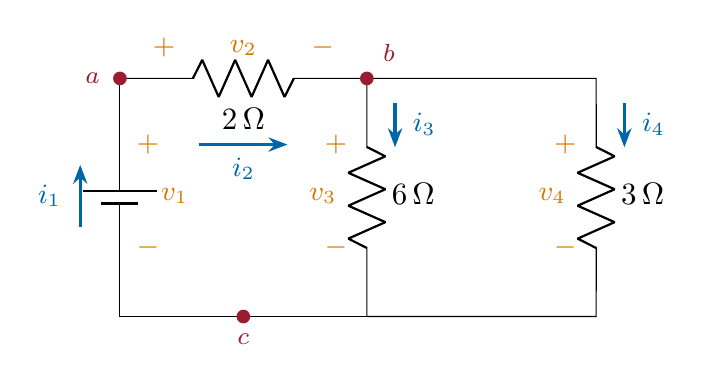
\begin{tikzpicture}[scale=1.12, transform shape]
  \draw (0,0) to[battery1, invert] (0,2.7);
  \draw (0,2.7) to[R, l_=$2\ohm$] (2.8,2.7);
  \draw (2.8,2.7) to[R, l=$6\ohm$] (2.8,0);
  \draw (2.8,2.7) -- (5.4,2.7) to[R, l=$3\ohm$] (5.4,0) -- (2.8,0);
  \draw (2.8,0) -- (0,0);
  \node[pol] at (0.32,1.95) {$+$}; \node[pol] at (0.32,0.78) {$-$};
  \node[pol] at (0.62,1.37) {$v_1$};
  \draw[iar] (-0.45,1.02) -- (-0.45,1.72); \node[ccur, font=\small] at (-0.8,1.37) {$i_1$};
  \node[pol] at (0.5,3.05) {$+$}; \node[pol] at (2.3,3.05) {$-$};
  \node[pol] at (1.4,3.05) {$v_2$};
  \draw[iar] (0.9,1.95) -- (1.9,1.95); \node[ccur, font=\small] at (1.4,1.68) {$i_2$};
  \node[pol] at (2.45,1.95) {$+$}; \node[pol] at (2.45,0.78) {$-$};
  \node[pol] at (2.3,1.37) {$v_3$};
  \draw[iar] (3.12,2.42) -- (3.12,1.92); \node[ccur, font=\small] at (3.45,2.18) {$i_3$};
  \node[pol] at (5.05,1.95) {$+$}; \node[pol] at (5.05,0.78) {$-$};
  \node[pol] at (4.9,1.37) {$v_4$};
  \draw[iar] (5.72,2.42) -- (5.72,1.92); \node[ccur, font=\small] at (6.05,2.18) {$i_4$};
  \fill[metured] (0,2.7) circle (2.2pt); \node[glab, left=3pt] at (0,2.7) {$a$};
  \fill[metured] (2.8,2.7) circle (2.2pt); \node[glab] at (3.05,2.99) {$b$};
  \fill[metured] (1.4,0) circle (2.2pt); \node[glab, below=2pt] at (1.4,0) {$c$};
\end{tikzpicture}
\end{center}

\subsection{Node, branch, loop}

Three words, all from Lecture~1, and every one of them is about the \emph{drawing}, not
about the components.

\begin{center}
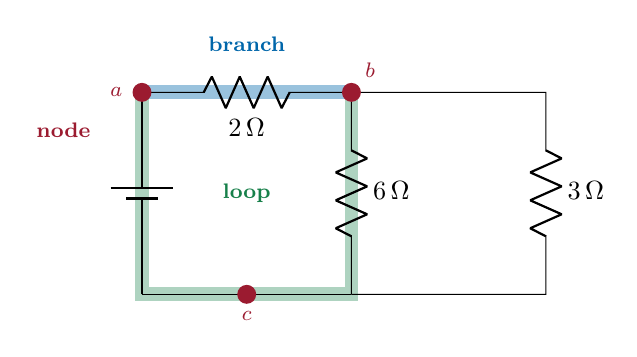
\begin{tikzpicture}[scale=0.95, transform shape]
  \draw[cpow!35, line width=5pt] (0,2.7) -- (0,0) -- (2.8,0) -- (2.8,2.7) -- (0,2.7);
  \draw[ccur!40, line width=5pt] (0,2.7) -- (2.8,2.7);
  \draw (0,0) to[battery1, invert] (0,2.7);
  \draw (0,2.7) to[R, l_=$2\ohm$] (2.8,2.7);
  \draw (2.8,2.7) to[R, l=$6\ohm$] (2.8,0);
  \draw (2.8,2.7) -- (5.4,2.7) to[R, l=$3\ohm$] (5.4,0) -- (2.8,0);
  \draw (2.8,0) -- (0,0);
  \fill[metured] (0,2.7) circle (3.6pt); \node[glab, left=4pt] at (0,2.7) {$a$};
  \fill[metured] (2.8,2.7) circle (3.6pt); \node[glab] at (3.05,2.99) {$b$};
  \fill[metured] (1.4,0) circle (3.6pt); \node[glab, below=3pt] at (1.4,0) {$c$};
  \node[font=\footnotesize\bfseries, text=ccur] at (1.4,3.35) {branch};
  \node[font=\footnotesize\bfseries, text=cpow] at (1.4,1.35) {loop};
  \node[font=\footnotesize\bfseries, text=metured] at (-1.05,2.2) {node};
\end{tikzpicture}
\end{center}

\begin{center}
\small
\begin{tabular}{@{}l l p{10.4cm}@{}}
\toprule
\textbf{Node}   & $n = 3$ & a connection point. Everything joined by ideal wire is
                  \emph{one} node, however far the drawing spreads it out.
                  Here: $a$, $b$, $c$.\\
\textbf{Branch} & $b = 4$ & one element, joining two nodes. Here: the source and the three
                  resistors.\\
\textbf{Loop}   & --- & a closed path that passes through no node twice. Here: the
                  left-hand one, the right-hand one, and the outer one.\\
\bottomrule
\end{tabular}
\end{center}

We will use $n$ for the number of nodes and $b$ for the number of branches throughout.

\subsection{What we do not know}
Each branch carries a \Vcol{voltage} and a \Icol{current}, and none of the eight is
known yet:
\[
  \underbrace{\Vcol{v_1},\ \Vcol{v_2},\ \Vcol{v_3},\ \Vcol{v_4}}_{\text{4 unknowns}}
  \qquad
  \underbrace{\Icol{i_1},\ \Icol{i_2},\ \Icol{i_3},\ \Icol{i_4}}_{\text{4 unknowns}}
  \qquad\Longrightarrow\qquad
  \boxed{\,2b = 8 \text{ unknown functions of } t\,}
\]

\subsection{Half the equations are easy}

Each element brings one equation of its own, a \textbf{terminal equation}. It describes
that element \emph{in isolation} and knows nothing about the rest of the circuit:
\[
  \Vcol{v_1} = 12\V, \qquad
  \Vcol{v_2} = 2\,\Icol{i_2}, \qquad
  \Vcol{v_3} = 6\,\Icol{i_3}, \qquad
  \Vcol{v_4} = 3\,\Icol{i_4} .
\]

\begin{center}
\small
\begin{tabular}{@{}l l l@{}}
\toprule
\textbf{Element} & \textbf{Symbol} & \textbf{Terminal equation}\\
\midrule
resistor             & $R$   & $\Vcol{v} = R\,\Icol{i}$\\
inductor             & $L$   & $\Vcol{v} = L\,d\Icol{i}/dt$\\
capacitor            & $C$   & $\Icol{i} = C\,d\Vcol{v}/dt$\\
ind.\ voltage source & $v_s$ & $\Vcol{v} = v_s(t)$, \ $\Icol{i}$ free\\
ind.\ current source & $i_s$ & $\Icol{i} = i_s(t)$, \ $\Vcol{v}$ free\\
\bottomrule
\end{tabular}
\end{center}

That is $b = 4$ equations for $2b = 8$ unknowns. \textbf{Exactly half.} And no amount of
staring at the elements will produce the other half: put the same four components together
differently and every current changes, while not one terminal equation does.

\subsection{The missing half comes from the wiring}

\begin{center}
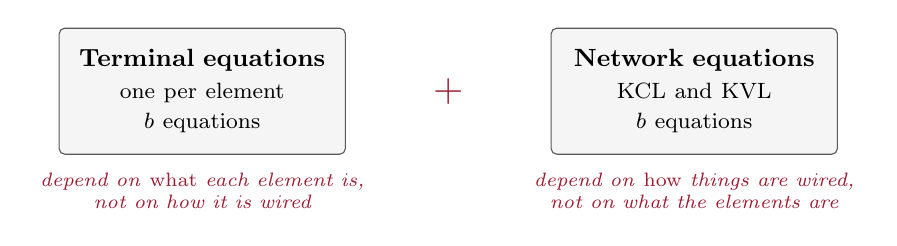
\begin{tikzpicture}[node distance=0.9cm]
  \node[blk, text width=3.4cm, minimum height=1.6cm] (t)
       {\textbf{Terminal equations}\\[2pt]\footnotesize
        one per element\\ \footnotesize $b$ equations};
  \node[blk, text width=3.4cm, minimum height=1.6cm, right=2.6cm of t] (n)
       {\textbf{Network equations}\\[2pt]\footnotesize
        KCL and KVL\\ \footnotesize $b$ equations};
  \node[below=3pt of t, font=\scriptsize\itshape, text=metured, text width=4.2cm, align=center]
       {depend on \emph{what} each element is,\\ not on how it is wired};
  \node[below=3pt of n, font=\scriptsize\itshape, text=metured, text width=4.2cm, align=center]
       {depend on \emph{how} things are wired,\\ not on what the elements are};
  \node[font=\Large, text=metured] at ($(t)!0.5!(n)$) {$+$};
\end{tikzpicture}
\end{center}

\begin{ideabox}[The whole strategy of circuit theory]
Cut the problem in two. The \textbf{elements} know nothing about the circuit they sit in;
the \textbf{interconnection} knows nothing about the elements it joins. Kirchhoff's two
laws are that second half, and this lecture is about them.\\[3pt]
Because they ignore the elements, KCL and KVL hold for \emph{every} lumped circuit ---
linear or nonlinear, time-invariant or time-varying, at DC or at $100\uni{MHz}$.
\end{ideabox}


%==============================================================
\section{Kirchhoff's Current Law}

\begin{definitionbox}{KCL}
For \textbf{every node} of a lumped circuit and at \textbf{every instant} $t$, the
algebraic sum of the currents \emph{leaving} the node is zero:
\[
  \sum_{k \,\in\, \text{node}} \pm\, \Icol{i_k(t)} \;=\; 0 ,
  \qquad
  \text{sign } + \text{ if the arrow points \emph{away} from the node.}
\]
Equivalently: \emph{what flows in, flows out.}
\end{definitionbox}

\textbf{Why.} A node is a junction of ideal wires; it has no volume and stores no charge.
If $q_{\text{node}}(t) = 0$ for all $t$, then charge conservation gives
\[
  \frac{dq_{\text{node}}}{dt} \;=\; \sum_{\text{in}} \Icol{i_k} - \sum_{\text{out}} \Icol{i_k} \;=\; 0 .
\]
So KCL is conservation of charge plus the lumped assumption from Lecture~1
(\emph{nothing piles up}).

\begin{center}
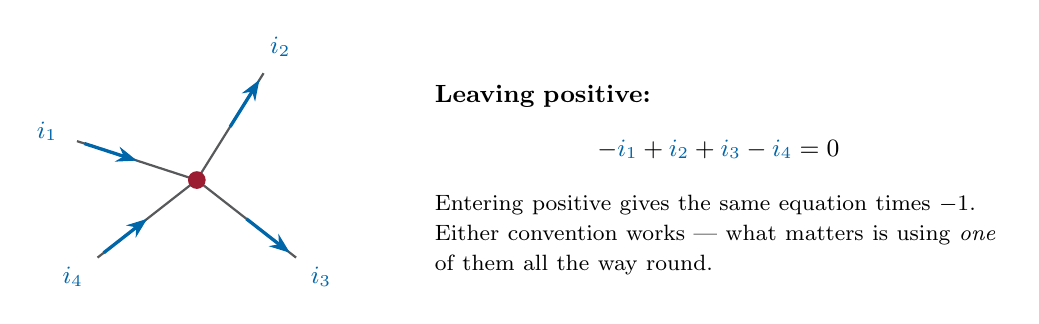
\begin{tikzpicture}[scale=1.0]
  \foreach \a in {162,58,-38,-142}{\draw[metugray, thick] (0,0) -- (\a:1.6);}
  \fill[metured] (0,0) circle (3.2pt);
  \draw[curarr] (162:1.50) -- (162:0.80);
  \draw[curarr] (58:0.80) -- (58:1.50);
  \draw[curarr] (-38:0.80) -- (-38:1.50);
  \draw[curarr] (-142:1.50) -- (-142:0.80);
  \node[ccur, font=\small] at (162:2.0) {$i_1$};
  \node[ccur, font=\small] at (58:2.0) {$i_2$};
  \node[ccur, font=\small] at (-38:2.0) {$i_3$};
  \node[ccur, font=\small] at (-142:2.0) {$i_4$};
  \node[font=\small, anchor=west, text width=7.2cm] at (2.9,0)
    {\textbf{Leaving positive:}
     \[ -\Icol{i_1} + \Icol{i_2} + \Icol{i_3} - \Icol{i_4} = 0 \]
     \footnotesize Entering positive gives the same equation times $-1$. Either
     convention works --- what matters is using \emph{one} of them all the way round.};
\end{tikzpicture}
\end{center}

\begin{examplebox}[Example 2.1 --- KCL at a node]
Four branches meet at a node with the reference arrows above. Measurements give
$\Icol{i_1} = 3\A$, $\Icol{i_2} = -2\A$ and $\Icol{i_3} = 6\A$. Find $\Icol{i_4}$.
\[
  -\Icol{i_1} + \Icol{i_2} + \Icol{i_3} - \Icol{i_4} = 0
  \;\Longrightarrow\;
  -3 + (-2) + 6 - \Icol{i_4} = 0
  \;\Longrightarrow\;
  \boxed{\Icol{i_4} = 1\A}
\]
Two lessons. The measured $\Icol{i_2} = -2\A$ enters the equation \emph{with its own sign};
we do not redraw the arrow. And the equation is written from the picture, not from any
idea of which way the charge ``really'' goes.
\end{examplebox}

\subsection{KCL on a closed surface}

Nothing in the argument above used the fact that the region enclosed was a single point.
Draw \emph{any} closed surface: if the charge inside it does not accumulate, the algebraic
sum of the currents crossing it is zero.

\begin{center}
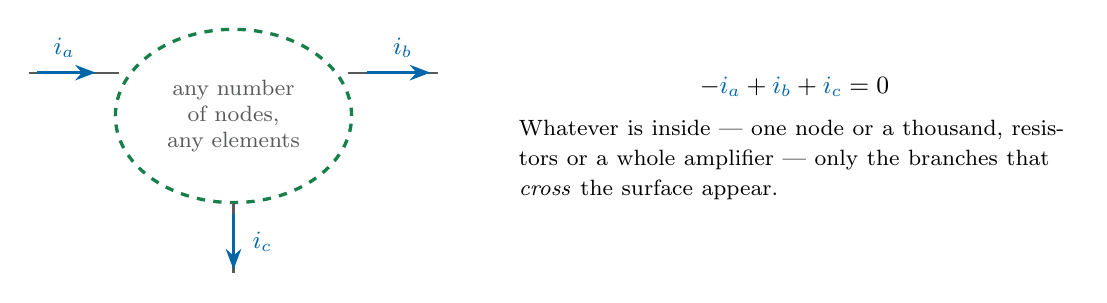
\begin{tikzpicture}[scale=1.0]
  \draw[surf] (0,0) ellipse (1.5cm and 1.1cm);
  \node[font=\footnotesize, text=metugray, align=center] at (0,0)
       {any number\\ of nodes,\\ any elements};
  \draw[metugray, thick] (-1.45,0.55) -- (-2.6,0.55);
  \draw[metugray, thick] (1.45,0.55) -- (2.6,0.55);
  \draw[metugray, thick] (0,-1.1) -- (0,-2.0);
  \draw[curarr] (-2.5,0.55) -- (-1.75,0.55);
  \draw[curarr] (1.7,0.55) -- (2.5,0.55);
  \draw[curarr] (0,-1.25) -- (0,-1.95);
  \node[ccur, font=\small, above] at (-2.15,0.62) {$i_a$};
  \node[ccur, font=\small, above] at (2.15,0.62) {$i_b$};
  \node[ccur, font=\small, right] at (0.12,-1.6) {$i_c$};
  \node[font=\small, anchor=west, text width=7.0cm] at (3.5,-0.2)
    {\[ -\Icol{i_a} + \Icol{i_b} + \Icol{i_c} = 0 \]
     \footnotesize Whatever is inside --- one node or a thousand, resistors or a whole
     amplifier --- only the branches that \emph{cross} the surface appear.};
\end{tikzpicture}
\end{center}

\begin{examplebox}[Example 2.2 --- two consequences of the surface form]
\textbf{(a) Series elements carry the same current.} Wrap a surface around the junction of
two elements joined end to end. Exactly two branches cross it, so
$\Icol{i_1} = \Icol{i_2}$: a chain of elements has \emph{one} current, and that is the
definition of ``in series''.
\vspace{2pt}

\begin{center}
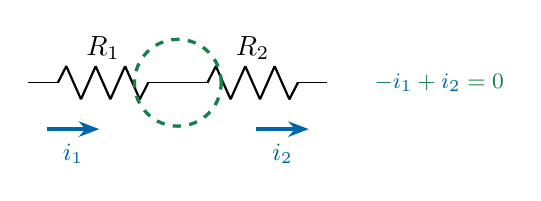
\begin{tikzpicture}[scale=0.95]
  \draw (0,0) to[R, l=$R_1$] (2.0,0) to[R, l=$R_2$] (4.0,0);
  \draw[surf] (2.0,0) circle (0.58cm);
  \draw[curarr] (0.25,-0.62) -- (0.95,-0.62);
  \draw[curarr] (3.05,-0.62) -- (3.75,-0.62);
  \node[ccur, font=\small] at (0.60,-0.95) {$i_1$};
  \node[ccur, font=\small] at (3.40,-0.95) {$i_2$};
  \node[font=\footnotesize, text=cpow, anchor=west] at (4.5,0) {$-\Icol{i_1}+\Icol{i_2}=0$};
\end{tikzpicture}
\end{center}
\vspace{-2pt}
\textbf{(b) A two-terminal box returns everything it is given.} Put the surface around an
entire sub-network reached by two wires: the current in at one terminal equals the current
out at the other, no matter how complicated the inside is. This is what lets us speak of
``\emph{the} current through'' a black box.
\end{examplebox}

\begin{cautionbox}[Two things KCL is not]
\begin{itemize}
  \item It is an equation about \textbf{one instant}. $\sum i_k(t) = 0$ holds for each $t$
        separately; nothing is averaged over time.
  \item It says nothing about voltages, resistances or power. Only topology and current.
\end{itemize}
\end{cautionbox}

%==============================================================
\section{Kirchhoff's Voltage Law}

\begin{definitionbox}{KVL}
For \textbf{every loop} of a lumped circuit and at \textbf{every instant} $t$, the
algebraic sum of the branch voltages around the loop is zero:
\[
  \sum_{k \,\in\, \text{loop}} \pm\, \Vcol{v_k(t)} \;=\; 0 ,
  \qquad
  \text{sign } + \text{ if you traverse the branch from } + \text{ to } - .
\]
Equivalently: \emph{go all the way round and you come back to where you started.}
\end{definitionbox}

\textbf{Why.} In a lumped circuit every node $j$ can be given a single number $e_j$, its
potential with respect to a chosen reference. A branch voltage is then a difference,
$\Vcol{v_k} = e_{(+)} - e_{(-)}$, and going round a loop $a \to b \to c \to a$ the sum
telescopes:
\[
  (e_a - e_b) + (e_b - e_c) + (e_c - e_a) \;=\; 0 .
\]
Energetically: carry a charge once around the loop and it ends where it began, so the net
energy exchanged per unit charge is zero. Like KCL, this is the lumped model at work ---
it needs assumption~(b), no changing magnetic field through the loop.\footnote{A
transformer breaks that assumption on purpose: the loop picks up a voltage belonging to no
element in the drawing. The cure is to draw the coupling as an element of its own, after
which KVL holds again exactly as written.}

\begin{center}
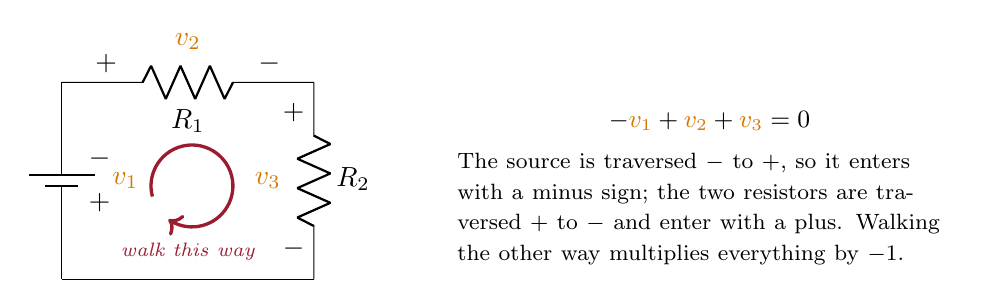
\begin{tikzpicture}[scale=1.0]
  \draw (0,0) to[battery1, invert, v_={\color{cvolt}$v_1$}] (0,2.5);
  \draw (0,2.5) to[R, l_=$R_1$, v^={\color{cvolt}$v_2$}] (3.2,2.5);
  \draw (3.2,2.5) to[R, l=$R_2$, v_={\color{cvolt}$v_3$}] (3.2,0);
  \draw (3.2,0) -- (0,0);
  \draw[metured, very thick, ->] (1.15,1.05) arc (195:-125:0.52);
  \node[font=\scriptsize\itshape, text=metured] at (1.6,0.35) {walk this way};
  \node[font=\small, anchor=west, text width=6.4cm] at (4.9,1.25)
    {\[ -\Vcol{v_1} + \Vcol{v_2} + \Vcol{v_3} = 0 \]
     \footnotesize The source is traversed $-$ to $+$, so it enters with a minus sign;
     the two resistors are traversed $+$ to $-$ and enter with a plus. Walking the other
     way multiplies everything by $-1$.};
\end{tikzpicture}
\end{center}

\begin{ideabox}[Voltage does not depend on the path]
KVL is the same statement as: \emph{the voltage between two nodes is the same whichever
way you go between them.} If path~1 gives $\Vcol{v_{ab}}$ and path~2 gives
$\Vcol{v'_{ab}}$, then path~1 followed by path~2 backwards is a loop, so
$\Vcol{v_{ab}} - \Vcol{v'_{ab}} = 0$. That is why ``the voltage across $R_2$'' is a
meaningful phrase and why node potentials exist at all.
\end{ideabox}

\begin{examplebox}[Example 2.3 --- one loop]
$v_s = 12\V$, $R_1 = 2\ohm$, $R_2 = 4\ohm$ in the figure above. With the loop current
$\Icol{i}$ taken clockwise, the terminal equations give
$\Vcol{v_2} = R_1 \Icol{i}$ and $\Vcol{v_3} = R_2 \Icol{i}$, and $\Vcol{v_1} = v_s$. KVL:
\[
  -12 + 2\Icol{i} + 4\Icol{i} = 0
  \;\Longrightarrow\;
  \boxed{\Icol{i} = 2\A}, \qquad \Vcol{v_2} = 4\V, \quad \Vcol{v_3} = 8\V .
\]
Check: $4 + 8 = 12\V$. The $12\V$ supplied is shared between the two resistors, the larger
one taking the larger share --- a fact we will soon turn into a formula.
\end{examplebox}

\subsection{A loop that is not a mesh, and what ``independent'' means}

\begin{examplebox}[Example 2.4 --- three loops, two equations]
Take the circuit of page~1 with $v_s = 12\V$, $R_1 = 2\ohm$, $R_2 = 6\ohm$, $R_3 = 3\ohm$.

\begin{center}
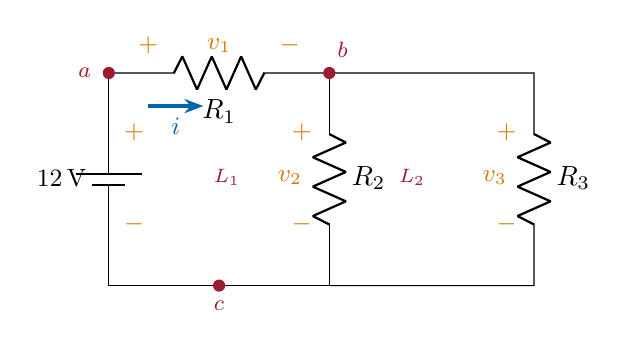
\begin{tikzpicture}[scale=1.0]
  \draw (0,0) to[battery1, invert] (0,2.7);
  \draw (0,2.7) to[R, l_=$R_1$] (2.8,2.7);
  \draw (2.8,2.7) to[R, l=$R_2$] (2.8,0);
  \draw (2.8,2.7) -- (5.4,2.7) to[R, l=$R_3$] (5.4,0) -- (2.8,0);
  \draw (2.8,0) -- (0,0);
  \node[pol] at (0.32,1.95) {$+$}; \node[pol] at (0.32,0.78) {$-$};
  \node[font=\small] at (-0.6,1.37) {$12\V$};
  \node[pol] at (0.5,3.05) {$+$}; \node[pol] at (2.3,3.05) {$-$};
  \node[pol] at (1.4,3.05) {$v_1$};
  \draw[iar] (0.50,2.28) -- (1.20,2.28); \node[ccur, font=\small] at (0.85,2.02) {$i$};
  \node[pol] at (2.45,1.95) {$+$}; \node[pol] at (2.45,0.78) {$-$};
  \node[pol] at (2.3,1.37) {$v_2$};
  \node[pol] at (5.05,1.95) {$+$}; \node[pol] at (5.05,0.78) {$-$};
  \node[pol] at (4.9,1.37) {$v_3$};
  \node[metured, font=\scriptsize\itshape] at (1.5,1.37) {$L_1$};
  \node[metured, font=\scriptsize\itshape] at (3.85,1.37) {$L_2$};
  \fill[metured] (0,2.7) circle (2.2pt); \node[glab, left=3pt] at (0,2.7) {$a$};
  \fill[metured] (2.8,2.7) circle (2.2pt); \node[glab] at (2.97,2.99) {$b$};
  \fill[metured] (1.4,0) circle (2.2pt); \node[glab, below=2pt] at (1.4,0) {$c$};
\end{tikzpicture}
\end{center}
\vspace{-4pt}
Three loops can be drawn: $L_1$, $L_2$, and the outer one $L_3 = L_1 \cup L_2$. Walking
each clockwise,
\[
  L_1: \; -12 + \Vcol{v_1} + \Vcol{v_2} = 0, \qquad
  L_2: \; -\Vcol{v_2} + \Vcol{v_3} = 0, \qquad
  L_3: \; -12 + \Vcol{v_1} + \Vcol{v_3} = 0 .
\]
The third is the sum of the first two: it is \emph{true}, but it is not \emph{new}. Adding
it to the system would gain nothing.
\vspace{3pt}

Note also what $L_2$ says on its own: $\Vcol{v_2} = \Vcol{v_3}$. Two elements joined at
\emph{both} ends always carry the same voltage --- there is a loop containing nothing else,
and KVL closes it. (Section~5 solves this circuit completely.)
\end{examplebox}

%==============================================================
\section{How many equations, and which ones?}

Recall from Section~1.1: $n$ is the number of \textbf{nodes}, $b$ the number of
\textbf{branches}. For the circuit of page~1, $n = 3$ and $b = 4$.

\begin{center}
\small
\begin{tabular}{@{}l c l@{}}
\toprule
\textbf{Source of equations} & \textbf{How many} & \textbf{Why that many}\\
\midrule
KCL, one per node          & $n - 1$      & the $n$-th is the sum of the others\\
KVL, one per loop          & $b - n + 1$  & $=\ell$, the independent loops\\[2pt]
\quad \textit{network equations} & $\mathbf{b}$ & \\
\midrule
terminal equations, one per element & $\mathbf{b}$ & \\
\midrule
\textbf{total} & $\mathbf{2b}$ & $=$ number of unknowns $v_k, i_k$\\
\bottomrule
\end{tabular}
\end{center}

Why is one KCL redundant? Add the node equations of \emph{every} node: each branch leaves
one node and enters another, so its current appears once with $+$ and once with $-$ and
cancels. The sum is $0 = 0$, so the $n$ equations carry only $n-1$ pieces of information.

For the running example: $n = 3$, $b = 4$, so $2$ independent KCL equations, $2$
independent KVL equations, $4$ terminal equations --- $8$ equations for the $8$ unknowns
$v_1..v_4$, $i_1..i_4$. We will soon turn this bookkeeping into systematic recipes (node and mesh
analysis) that never write all $2b$ equations at once.

%==============================================================
\begin{cautionbox}[Some diagrams have no solution at all]
KCL and KVL do not only solve circuits; they also decide which drawings \emph{mean}
anything.
\begin{itemize}
  \item Connect an ideal $5\V$ source directly across an ideal $9\V$ source. That loop
        contains nothing else, so KVL reads $5 - 9 = 0$. False --- and no choice of
        currents can repair it.
  \item Put an ideal $2\A$ source in a chain with an ideal $3\A$ source. KCL at the node
        between them reads $2 = 3$. False again, whatever the voltages do.
\end{itemize}
Neither is an algebra mistake. The equations are contradictory, so the diagram describes
no circuit at all. What has gone wrong is the \emph{model}: an ideal source promises to
hold its value no matter what current or voltage that costs, and two such promises can
simply disagree.\\[3pt]
Real components never promise that much. Give each battery its internal resistance and the
equations become consistent again --- and then tell you that a very large current
circulates. Sometimes that is a harmless detail; sometimes it is the reason one of the
batteries makes smoke.
\end{cautionbox}

%==============================================================
\section{Solving the circuit of page 1}

Collect everything. Four terminal equations, two KCL, two KVL --- eight equations, eight
unknowns, and no method beyond substitution.

\begin{center}
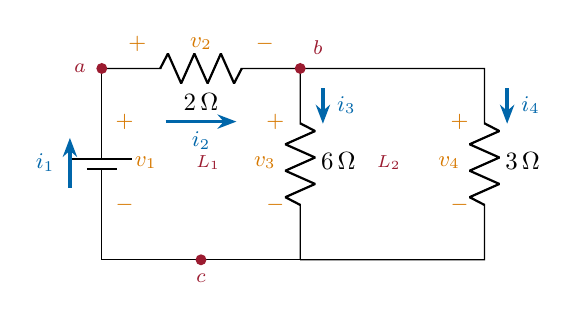
\begin{tikzpicture}[scale=0.9, transform shape]
  \draw (0,0) to[battery1, invert] (0,2.7);
  \draw (0,2.7) to[R, l_=$2\ohm$] (2.8,2.7);
  \draw (2.8,2.7) to[R, l=$6\ohm$] (2.8,0);
  \draw (2.8,2.7) -- (5.4,2.7) to[R, l=$3\ohm$] (5.4,0) -- (2.8,0);
  \draw (2.8,0) -- (0,0);
  \node[pol] at (0.32,1.95) {$+$}; \node[pol] at (0.32,0.78) {$-$};
  \node[pol] at (0.62,1.37) {$v_1$};
  \draw[iar] (-0.45,1.02) -- (-0.45,1.72); \node[ccur, font=\small] at (-0.8,1.37) {$i_1$};
  \node[pol] at (0.5,3.05) {$+$}; \node[pol] at (2.3,3.05) {$-$};
  \node[pol] at (1.4,3.05) {$v_2$};
  \draw[iar] (0.9,1.95) -- (1.9,1.95); \node[ccur, font=\small] at (1.4,1.68) {$i_2$};
  \node[pol] at (2.45,1.95) {$+$}; \node[pol] at (2.45,0.78) {$-$};
  \node[pol] at (2.3,1.37) {$v_3$};
  \draw[iar] (3.12,2.42) -- (3.12,1.92); \node[ccur, font=\small] at (3.45,2.18) {$i_3$};
  \node[pol] at (5.05,1.95) {$+$}; \node[pol] at (5.05,0.78) {$-$};
  \node[pol] at (4.9,1.37) {$v_4$};
  \draw[iar] (5.72,2.42) -- (5.72,1.92); \node[ccur, font=\small] at (6.05,2.18) {$i_4$};
  \node[metured, font=\scriptsize\itshape] at (1.5,1.37) {$L_1$};
  \node[metured, font=\scriptsize\itshape] at (4.05,1.37) {$L_2$};
  \fill[metured] (0,2.7) circle (2.2pt); \node[glab, left=3pt] at (0,2.7) {$a$};
  \fill[metured] (2.8,2.7) circle (2.2pt); \node[glab] at (3.05,2.99) {$b$};
  \fill[metured] (1.4,0) circle (2.2pt); \node[glab, below=2pt] at (1.4,0) {$c$};
\end{tikzpicture}
\end{center}
\vspace{-4pt}

\begin{center}
\small
\begin{tabular}{@{}l@{\hspace{1.4em}}l@{\hspace{1.4em}}l@{}}
\toprule
\textbf{4 terminal equations} & \textbf{2 KCL ($n-1$)} & \textbf{2 KVL ($b-n+1$)}\\
\midrule
$\Vcol{v_1} = 12$          & node $a$: \ $-\Icol{i_1}+\Icol{i_2} = 0$ & $L_1$: \ $-\Vcol{v_1}+\Vcol{v_2}+\Vcol{v_3} = 0$\\
$\Vcol{v_2} = 2\,\Icol{i_2}$ & node $b$: \ $-\Icol{i_2}+\Icol{i_3}+\Icol{i_4} = 0$ & $L_2$: \ $-\Vcol{v_3}+\Vcol{v_4} = 0$\\
$\Vcol{v_3} = 6\,\Icol{i_3}$ & & \\
$\Vcol{v_4} = 3\,\Icol{i_4}$ & & \\
\bottomrule
\end{tabular}
\end{center}

Eliminate in the order the equations suggest. $L_2$ gives $6\Icol{i_3} = 3\Icol{i_4}$, so
$\Icol{i_4} = 2\Icol{i_3}$. KCL at $b$ then gives $\Icol{i_2} = \Icol{i_3} + \Icol{i_4}
= 3\Icol{i_3}$. Substituting into $L_1$,
\[
  -12 + 2\Icol{i_2} + 6\Icol{i_3} = 0
  \quad\text{with}\quad \Icol{i_3} = \tfrac13\Icol{i_2}
  \qquad\Longrightarrow\qquad
  -12 + 2\Icol{i_2} + 2\Icol{i_2} = 0 .
\]
Hence
\[
  \Icol{i_1} = \Icol{i_2} = 3\A, \quad \Icol{i_3} = 1\A, \quad \Icol{i_4} = 2\A,
  \qquad
  \Vcol{v_1} = 12\V, \quad \Vcol{v_2} = 6\V, \quad \Vcol{v_3} = \Vcol{v_4} = 6\V .
\]

\begin{ideabox}[A free check: power must balance]
The source delivers $12 \times 3 = 36\W$; the resistors absorb
$2(3)^2 + 6(1)^2 + 3(2)^2 = 18 + 6 + 12 = 36\W$. So \Pcol{$\sum_k p_k = 0$}, as Lecture~1
promised. One line, and it catches most sign errors.
\end{ideabox}

The eight-equation system always works --- it is essentially what a circuit simulator
solves --- but it is slow by hand, and it grows fast: a circuit with thirty branches would
need sixty equations. We will soon learn much better ways of getting the same answer,
which write only a handful of equations and still satisfy KCL and KVL automatically.

%==============================================================
\section*{Summary}
\addcontentsline{toc}{section}{Summary}

\begin{center}
\small
\begin{tabular}{@{}l l l@{}}
\toprule
\textbf{Law} & \textbf{Statement} & \textbf{Rests on}\\
\midrule
KCL & $\sum \pm \Icol{i_k} = 0$ at every node, every instant
    & conservation of charge; nothing piles up\\
KVL & $\sum \pm \Vcol{v_k} = 0$ round every loop, every instant
    & node potentials exist; no stray flux\\
\bottomrule
\end{tabular}
\end{center}

\begin{itemize}
  \item A circuit gives $2b$ unknowns and $2b$ equations: $b$ \textbf{terminal} equations
        (what the elements are) and $b$ \textbf{network} equations,
        $n-1$ from KCL and $b-n+1$ from KVL (how they are wired).
  \item KCL holds on \textbf{any closed surface}, not only at a node. Elements joined end
        to end carry one current; a two-terminal box returns what it takes.
  \item KVL is the statement that \textbf{voltage does not depend on the path}. Elements
        joined at both ends carry one voltage.
  \item Signs come from the \emph{reference} arrows and polarities you drew, never from a
        guess about which way things really go.
  \item Neither law knows anything about the elements: both hold for nonlinear and
        time-varying circuits exactly as written.
\end{itemize}

\subsection*{Reading}
\begin{itemize}
  \item Alexander \& Sadiku, \emph{Fundamentals of Electric Circuits}, Chapter~2.
  \item Chua, Desoer \& Kuh, \emph{Linear and Nonlinear Circuits}, Chapter~2.
  \item Lecture notes and videos of Prof.\ Emre Tuna,
        \href{https://users.metu.edu.tr/etuna/ee201/}{\texttt{users.metu.edu.tr/etuna/ee201}}
        --- Lecture~2 video: network and terminal equations $6{:}50$, KCL $8{:}35$,
        KVL $18{:}55$.
\end{itemize}

\end{document}
